\section{Detecting Anomalous Transactions using KDE}
\subsection{Designing a custom KDE Class}
\begin{lstlisting}[language=Python, caption={Python code to implement \texttt{EpanechnikovKDE} class}, label=lst:epanechnikovkde]
class EpanechnikovKDE:
    def __init__(self, bandwidth=1.0):
        self.bandwidth = bandwidth
        self.data = None

    def fit(self, data):
        """Fit the KDE model with the given data."""
        self.data = data

    def epanechnikov_kernel(self, x, xi):
        """Epanechnikov kernel function."""
        a = np.linalg.norm((x - xi) / self.bandwidth, axis=-1)
        return np.where(a <= 1, (2 / np.pi) * (1 - a**2), 0)[()]

    def evaluate(self, x):
        """Evaluate the KDE at point x."""
        return self.epanechnikov_kernel(x, self.data).mean() / self.bandwidth**2
\end{lstlisting}

\subsection{Estimating Distribution of Transactions}
\vspace{-20pt}
\begin{figure}[H]
	\centering
	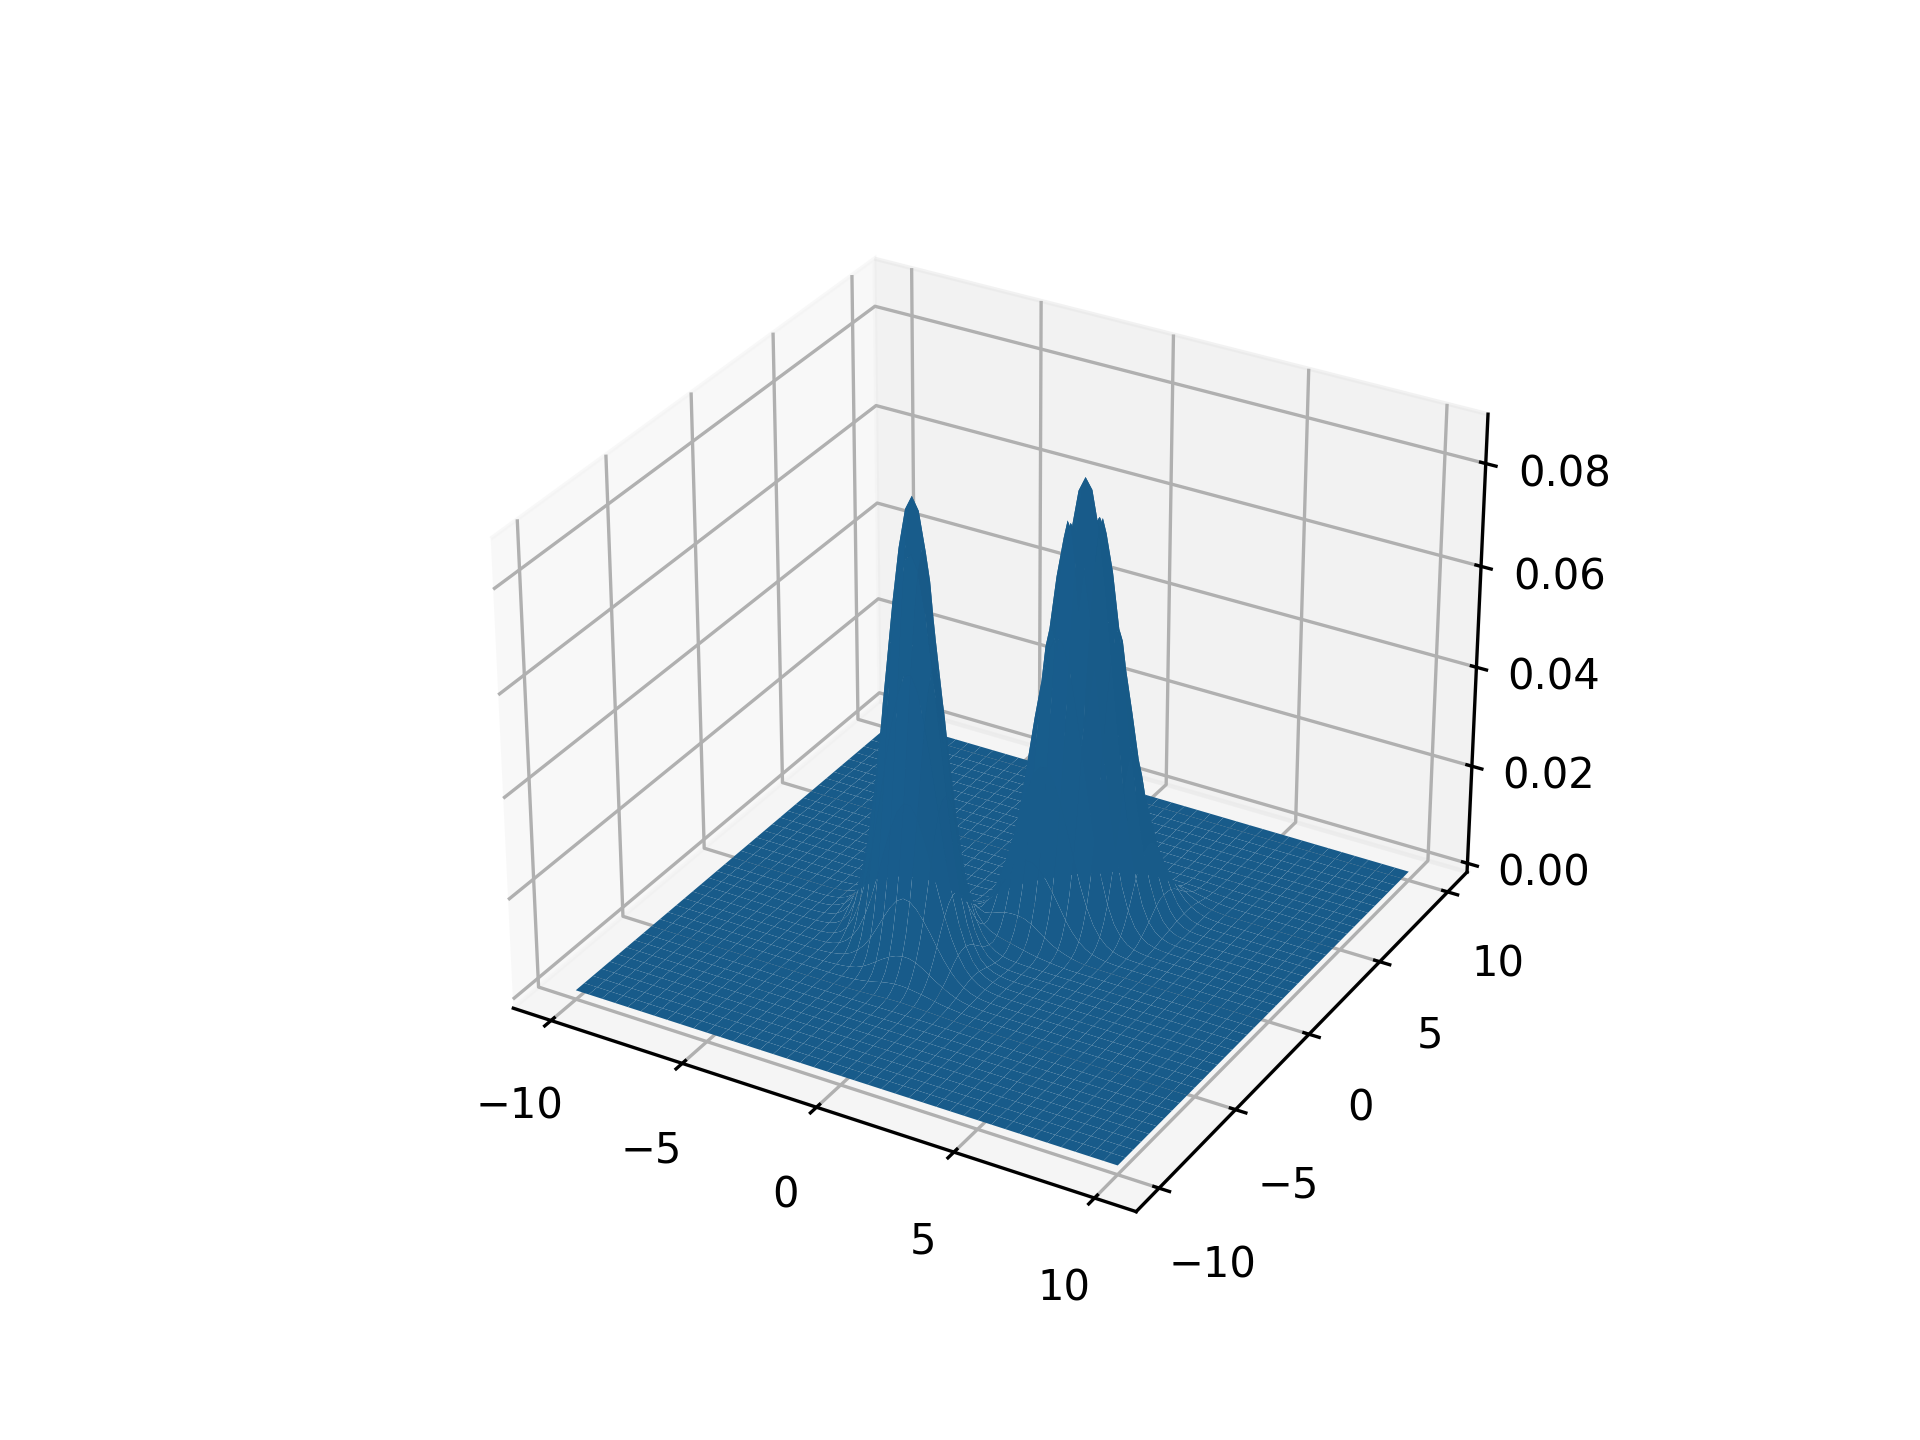
\includegraphics[width=0.6\textwidth]{images/2/transaction_distribution.png}
	\caption{Probability density of transactions}
\end{figure}
The resulting distribution has 2 modes, as seen in the plot.
